\documentclass[9pt]{beamer}

%!TEX root = ../notas_de_clase.tex

%preamble

%language
\usepackage[spanish,es-nodecimaldot]{babel}
\usepackage[utf8]{inputenc}
\usepackage{apacite}
\usepackage[absolute,overlay]{textpos}

%packages
\usepackage[Algoritmo]{algorithm}
\usepackage{algorithmicx}
\usepackage[noend]{algpseudocode}
\usepackage{mathtools}
\setlength {\marginparwidth}{2cm}
\usepackage{todonotes}
\usepackage{amsbsy}
\usepackage{amssymb}
\usepackage{amsmath,bm}
\usepackage{dsfont}

\usepackage{comment}

\usepackage{xcolor}
\providecommand{\sred}[1]{\textcolor{red}{#1}}
\providecommand{\sblue}[1]{\textcolor{blue}{#1}}
\providecommand{\red}[1]{\textcolor{red}{\text{#1}}}
\providecommand{\blue}[1]{\textcolor{blue}{\text{#1}}}
\providecommand{\redb}[1]{\textcolor{red}{\textbf{#1}}}
\providecommand{\blueb}[1]{\textcolor{blue}{\textbf{#1}}}
\usepackage{graphicx}
\usepackage{fancybox}
\usepackage{booktabs}
\usepackage{caption}
\usepackage{float}
%\usepackage[longend,ruled,algochapter,linesnumbered,lined,boxed,commentsnumbered,spanish]{algorithm2e}
%\usepackage[algo2e]{algorithm2e}
\usepackage{amssymb}
\usepackage{amstext}
\usepackage{bm}
\usepackage{wrapfig}
\usepackage{subcaption} % para_unsupervised_chapter

%formatting

\usepackage[export]{adjustbox}

%caption para figuras
\captionsetup[figure]{width=.8\linewidth, font=small,labelfont={bf},name={Fig.},labelsep=period}
\captionsetup[table]{width=.8\linewidth,font=small,labelfont={bf},name={Tabla},labelsep=period}



\ifx\byn\undefined
    \definecolor{my_blue}{HTML}{C2D5FF}
    \definecolor{my_red}{HTML}{FFC2C2}
    \definecolor{my_yellow}{HTML}{FFFFE0}
\else
    \definecolor{my_blue}{HTML}{FFFFFF}
    \definecolor{my_red}{HTML}{FFFFFF}
    \definecolor{my_yellow}{HTML}{FFFFFF}
\fi


\usepackage[framemethod=TikZ]{mdframed}
\mdfdefinestyle{discusion}{%
    %linecolor=black,
    %outerlinewidth=0pt,
    roundcorner=0pt,
    innertopmargin=5pt,
    innerbottommargin=5pt,
    innerrightmargin=20pt,
    innerleftmargin=20pt,
    backgroundcolor=my_blue}

\colorlet{Green}{green!90}


\mdfdefinestyle{ejemplo}{%
    %linecolor=black,
    %outerlinewidth=0pt,
    roundcorner=0pt,
    innertopmargin=5pt,
    innerbottommargin=5pt,
    innerrightmargin=20pt,
    innerleftmargin=20pt,
    backgroundcolor=my_yellow}


\mdfdefinestyle{pendiente}{%
    style = discusion, 
    backgroundcolor=my_red}


\RequirePackage{url}



%definitions
\def\td{{\text d}}
\def\cN{{\mathcal N}}
\def\cX{{\mathcal X}} 
\def\cC{{\mathcal C}} 
\def\N{{\mathbb N}}
\def\d{{\text d}}
\def\datos{{\mathcal D}}
\def\eye{{\mathbb I}}
\def\ssum{{\scriptstyle\sum}}
\def\bepsilon{{\bm \epsilon}}
\def\tx{\tilde{x}}
\def\tX{\tilde{X}}
\def\thetaMAP{\theta_\text{MAP}}
\newcommand{\gp}{\ensuremath{\mathcal{GP}}}
\newcommand{\pr}{\ensuremath{\mathbb{P}}}
\newcommand{\x}{\ensuremath{\mathbf{x}}}
\newcommand{\z}{\ensuremath{\mathbf{z}}}
\newcommand{\cvector}{\ensuremath{\mathbf{c}}}
\newcommand{\e}{\ensuremath{\mathbf{e}}}
\newcommand{\y}{\ensuremath{\mathbf{y}}}
\newcommand{\bx}{\ensuremath{\textcolor{blue}{X}}}
\newcommand{\by}{\ensuremath{\textcolor{blue}{Y}}}
\newcommand{\rx}{\ensuremath{\textcolor{red}{X_*}}}

\newcommand{\R}{\mathbb{R}}
\newcommand{\norm}[1]{\left\lVert#1\right\rVert}




\DeclareMathOperator*{\argmax}{arg\,max}
\DeclareMathOperator*{\argmin}{arg\,min}
\DeclareMathOperator{\E}{\mathbb{E}}
\DeclareMathOperator{\V}{\mathbb{V}}
\DeclareMathOperator{\KL}{\text{KL}}
\DeclareMathOperator{\MVN}{\text{MVN}}
\newcommand\deq{\stackrel{\mathclap{\normalfont\mbox{\tiny def}}}{=}}
%\newcommand{\E}[1]{\mathbb E \left[#1\right]}
\newcommand{\trace}[1]{\text{Tr} \left[#1\right]}


\usepackage{amsthm}

%-------------------------------------------
% Newtheorem
%-------------------------------------------
\newtheorem{axioma}{\textcolor{red}{Axioma}}
\newtheorem{definicion}{Definición}
\newtheorem*{notacion}{Notación}
\newtheorem{teorema}{Teorema}
\newtheorem{corolario}{Corolario}
\newtheorem{lema}{Lema}
\newtheorem{lemaZ}{\textcolor{red}{Lema}}
\newtheorem{propiedad}{Propiedad:}
\newtheorem{proposicion}{Proposición:}
\newtheorem*{observacion}{Observación}
\newtheorem*{comentario}{Comentario}
\newtheorem*{ejemplo}{Ejemplo}
\newtheorem*{resultado}{Resultado}
\newtheorem*{propuesto}{Ejercicio propuesto}
\newtheorem*{demostracion}{Demostración} % No se usa, usar \begin{proof}\end{proof} que son por default.

%listing paackage para código
\usepackage{listings}
\usepackage{xcolor}
 
\definecolor{codegreen}{rgb}{0,0.6,0}
\definecolor{codegray}{rgb}{0.5,0.5,0.5}
\definecolor{codepurple}{rgb}{0.58,0,0.82}
\definecolor{backcolour}{rgb}{0.95,0.95,0.92}
 
\lstdefinestyle{mystyle}{
    xleftmargin=0.15\textwidth,
    linewidth=0.8\textwidth,
    backgroundcolor=\color{backcolour},   
    commentstyle=\color{codegreen},
    keywordstyle=\color{magenta},
    numberstyle=\tiny\color{codegray},
    stringstyle=\color{codepurple},
    basicstyle=\ttfamily\footnotesize,
    breakatwhitespace=true,         
    breaklines=true,                 
    captionpos=b,                    
    keepspaces=true,                 
    numbers=left,                    
    numbersep=5pt,                  
    showspaces=false,                
    showstringspaces=false,
    showtabs=false,                  
    tabsize=2
}
 
\lstset{style=mystyle}

\numberwithin{equation}{section}

\usetheme{simple}
\usepackage{tikz}

\title{Clase 1: Introducción}
\subtitle{MDS7203 Modelos Generativos Profundos}
\date{7 de agosto de 2023}
\author{Felipe Tobar \\ Cristóbal Alcázar - Camilo Carvajal Reyes}  
\titlegraphic{
\begin{tikzpicture}[remember picture, overlay]
    \node[opacity=1.0, at=(current page.center)] {
\includegraphics[width=\paperwidth,height=\paperheight]{diapositivas/img/presentacion_plantilla_4_fondo_blanco-celeste.png}};
\end{tikzpicture}
\begin{figure}[htp] 
    \centering
        
\includegraphics[width=0.15\textwidth]{img/Uchile.pdf}%
        \hspace{1cm}
        \includegraphics[width=0.15\textwidth]{diapositivas/img/IDIA.png}
\end{figure}
}
\institute{Iniciativa de Datos e Inteligencia Artificial\\Universidad de Chile}

\begin{document}
\begin{frame}
  \titlepage
\end{frame}

\begin{frame}
    \frametitle{Tabla de contenidos}
    \tableofcontents
\end{frame}


\section{Logística y presentación del curso}
\begin{frame}
    \frametitle{Tabla de contenidos}
    \tableofcontents[currentsection]
\end{frame}

\subsection{Requisitos del curso}
\begin{frame}{Requisitos del curso}
    \begin{itemize}
        \item Requisitos del curso: Aprendizaje de Máquinas (cualquier versión) o Simulación Estocástica. También es posible pedirlo por autorización.
        \item Se requiere manejo básico en estadística / aprendizaje de máquinas
        \item Necesitarán conocimiento en probabilidades y cálculo, más precisamente conocer:
        \begin{itemize}
            \item Optimización con descenso de gradiente (y como consecuencia derivadas)
            % Gradients, gradient-descent optimization, backpropagation
            \item \textit{Backpropagation}
            \item Variables aleatorias, independencia e independencia condicional
            % Random variables, independence, conditional independence
            \item Teorema de Bayes, regla de la cadena y cambio de variables
            % Bayes rule, chain rule, change of variables formulas
        \end{itemize}
        \item Es importante que se manejen bien en \textit{python}.
    \end{itemize}
\end{frame}


\subsection{Organización del curso}
\begin{frame}{Organización del curso}

\begin{itemize}
  \item 2 clases por semana de 1.5 horas: lunes y viernes de 10:15 a 11:45 
  \item En general:
  \begin{itemize}
    \item Se espera que estudien el material de antemano
    \item 2 módulos teóricos
    \item 2 módulos de laboratorio (trabajo dirigido)
  \end{itemize}
  \item Sala: por definir
  \item Evaluaciones: 
  \begin{itemize}
    \item Quiz para evaluar conceptos básicos
    \item Laboratorios individuales, evaluación por trabajo en clases y entrega final
    \item Proyecto final
    \item color{red}$NF = NQ*0.15 + NL*0.45 + NP*0.4 $\color{black}
  \end{itemize}
  \item Además de Ucursos, la página con el material del curso es: \href{https://github.com/GAMES-UChile/Curso-Modelos-Generativos-Profundos}{\tt https://github.com/GAMES-UChile/Curso-Modelos-Generativos-Profundos}
  \item Canal de consultas oficial es el foro de U-cursos
\end{itemize}

\end{frame}


\section{Introducción a Modelos Generativos}
\begin{frame}
    \frametitle{Tabla de contenidos}
    \tableofcontents[currentsection]
\end{frame}

\subsection{Modelos Discriminativos}
\begin{frame}{Modelos Discriminativos}
    Para un modelo discriminativo el objetivo será tener una manera de decidir entre miembros de distintas clases.
    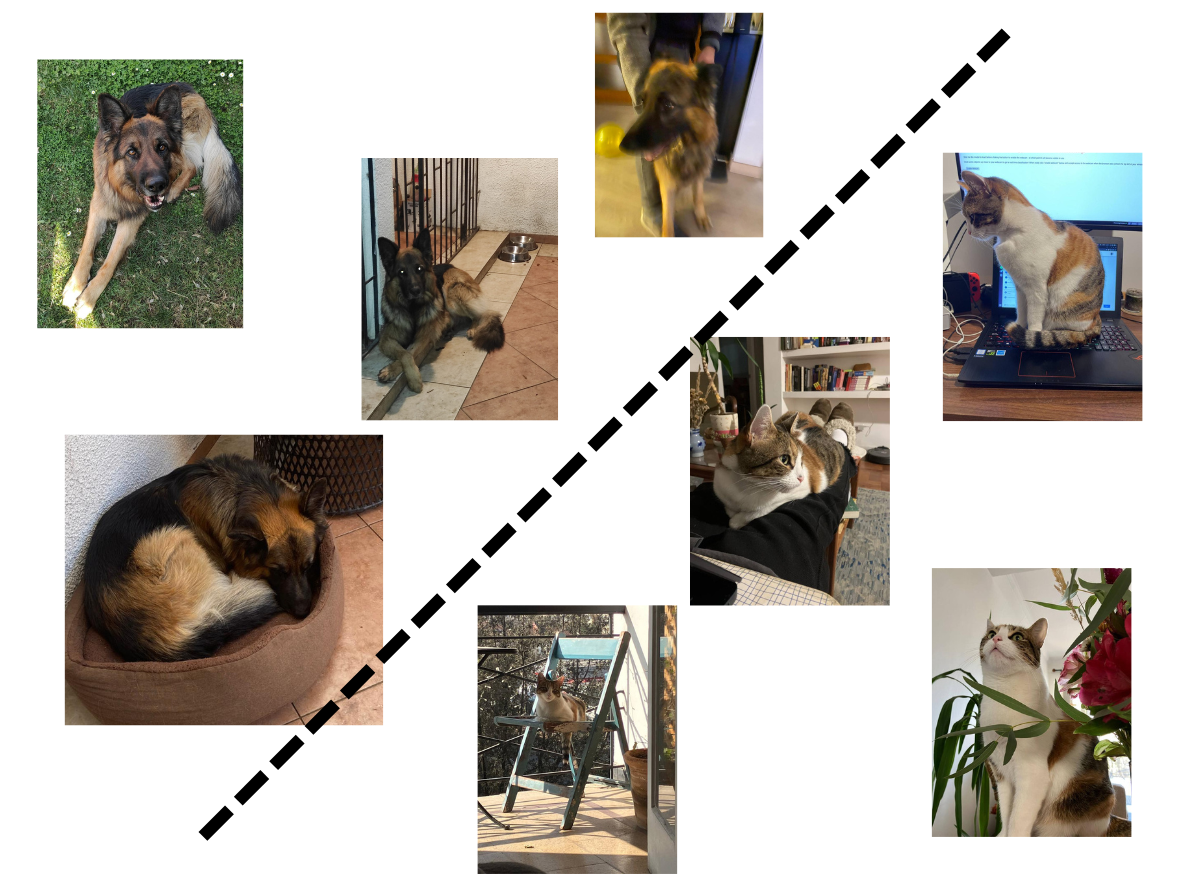
\includegraphics[width=0.85\textwidth]{diapositivas/img/discriminativo.png}
\end{frame}

\subsection{Modelos Generativos}
\begin{frame}{Modelo Generativo}
    En el caso de un modelo generativo, nuestro objetivo es modelar la estructura de los datos.\\
    \centering
    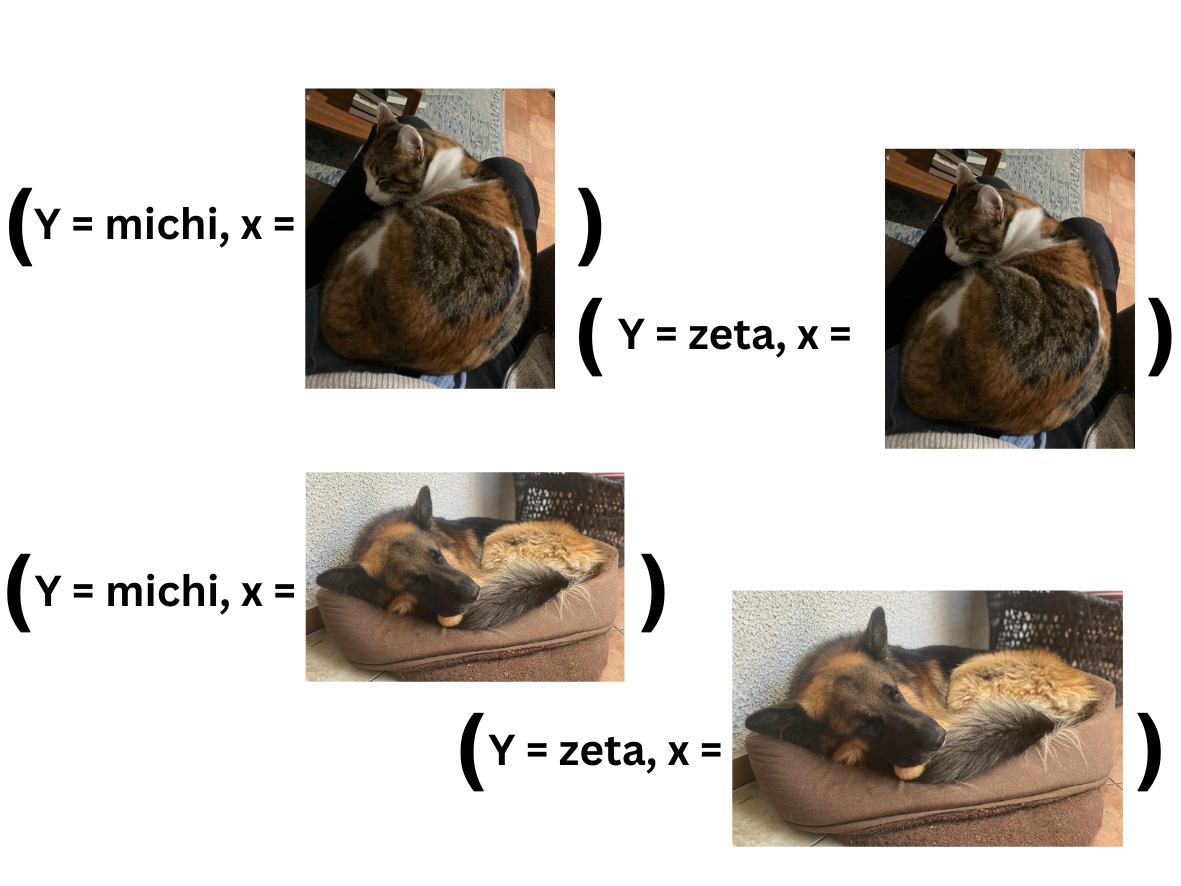
\includegraphics[width=0.85\textwidth]{diapositivas/img/generativo.png}
\end{frame}

\begin{frame}{Modelo Generativo}
    \only<1,4>{En el caso Gaussiano podíamos ajustar los parámetros que definen nuestra distribución de modo que se maximizara la log-verosimilitud.}
    \only<2>{
    \centering
    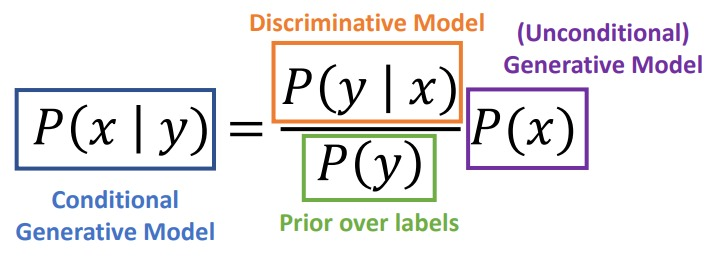
\includegraphics[width=0.65\textwidth]{diapositivas/img/conditional_generative.jpeg}
    }
    \only<3>{
    \centering
    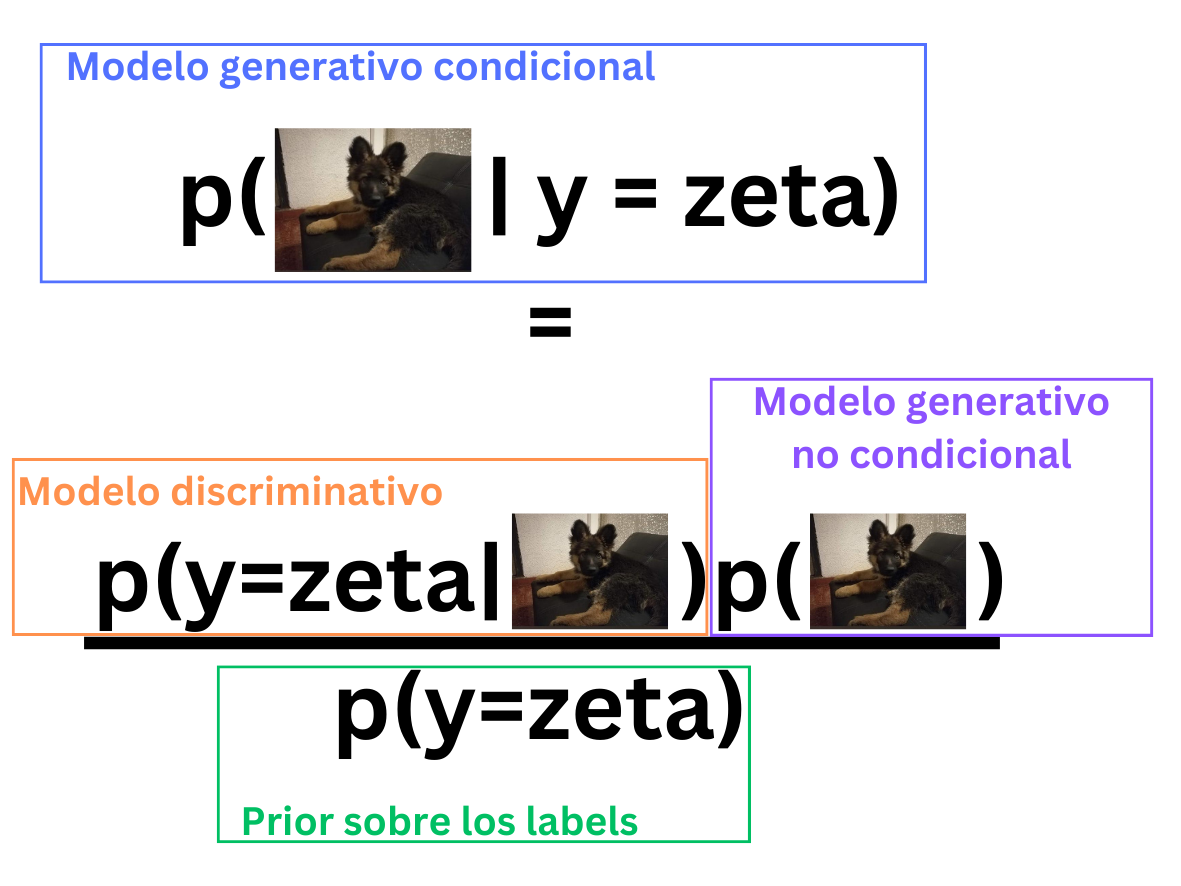
\includegraphics[width=0.95\textwidth]{diapositivas/img/generativo_condicional_zeta.png}
    }
    \only<4>{
    \newparagraph Sin embargo en general las distribuciones Gaussianas no logran reflejar la complejidad intrínseca de los datos. Muchos de los modelos que estudiaremos en este curso intentarán solucionar esta y otras limitaciones, pero manteniendo la capacidad de samplear nuevos puntos de datos.
    }
\end{frame}


\subsection{Ejemplos de Modelos Generativos}

\begin{frame}{Ejemplos de Modelos Generativos}
    \only<1>{
    \textbf{\textbf{Modelos basados en energía}}\\
    En este caso trataremos de modelar la densidad al considerar:
    $$ p_\theta(x) = \frac{\tilde p_\theta(x)}{Z_\theta} = \frac{e^{-E_\theta(x)}}{Z_\theta} \,,$$
    donde a $E_\theta:\mathbb{R}\to \mathbb{R}$ 
    se le llama la función de energía. La analogía es: mientras menos energía tenga, más probable serán un punto de dato. Por otro lado, $Z_\theta$ es simplemente un denominador que normaliza, que en general se considera intratable. Este tipo de modelamiento es flexible pero samplear requiere escoger muestreos con baja energía usando métodos de MCMC, lo cual a veces lleva a una disminución en calidad.
    }
    \only<2>{\textbf{\textbf{Autoencoders variacionales} (VAE)}\\
    Los VAEs modelan la distribución ajustando una red codificafora (\textit{encoder}) que mapea los datos de input a un espacio latente, y una red decodificadora (\textit{decoder}) que reconstruye el input usando muestreos del espacio latente. Esto captura la estructura subyacente y permite el sampleo desde la distribución aprendida dentro del espacio latente. \footnote{Fuente de la imagen: \url{https://lilianweng.github.io/posts/2018-08-12-vae/}}
    \begin{figure}
        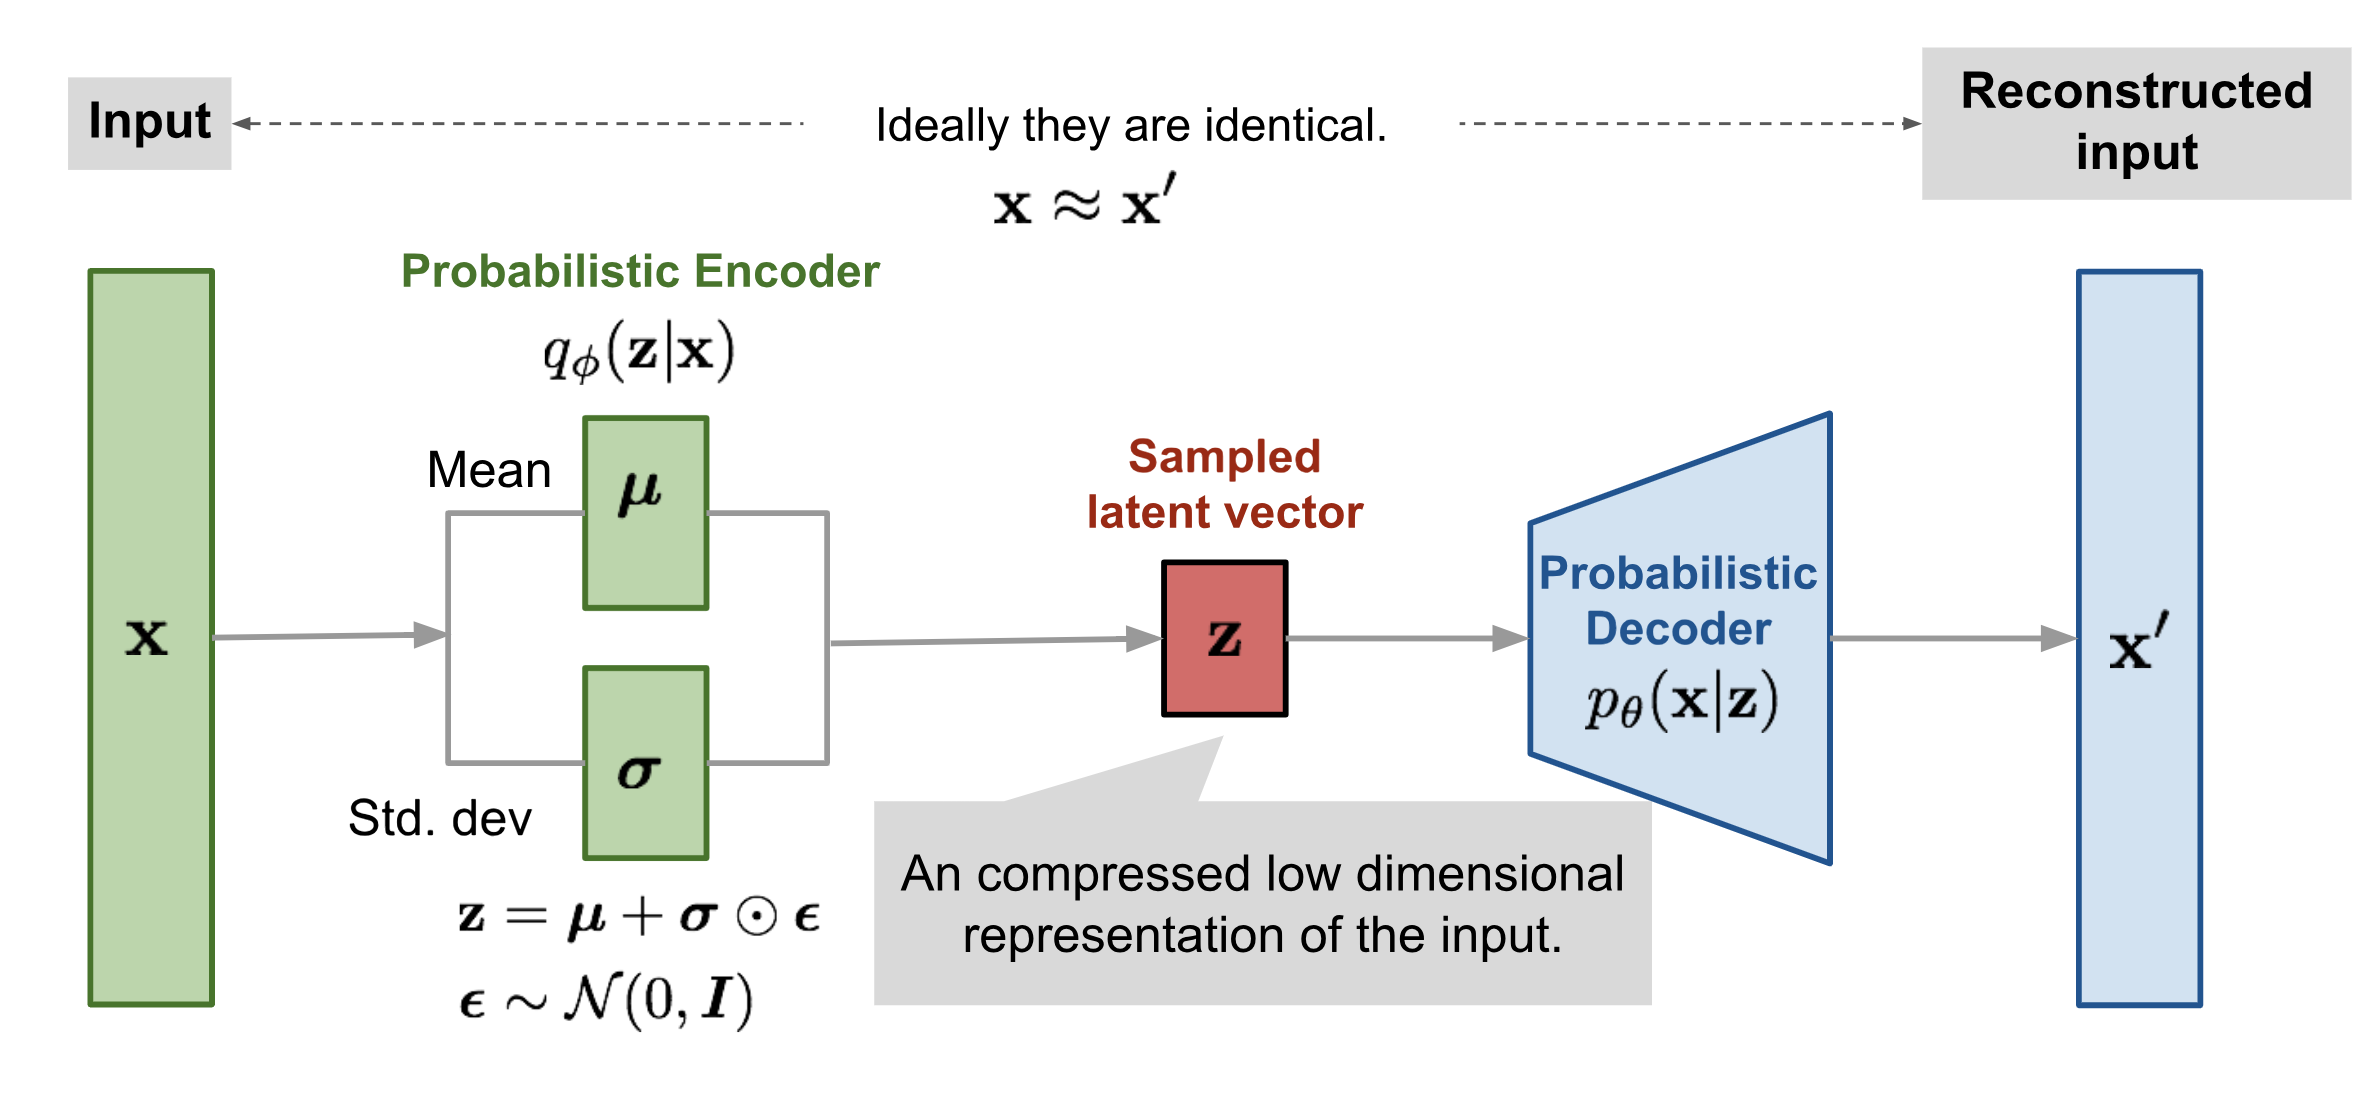
\includegraphics[width=0.85\textwidth]{diapositivas/img/vae-gaussian-lilian-weng-diagram.png}
    \end{figure}}
    \only<3>{\textbf{\textbf{Flujos normalizantes}}\\
    Un modelo de flujos normalizantes (\textit{normalizing flows}) modela la distribución de los datos aplicando una secuencia de transformaciones invertiles a una base de distribuciones simples, como Gaussianas. Esto permite al modelo aprender y generar muestras de distribuciones complejas al transformar los datos de forma iterativa y actuailizar la densidad de probabilidad usando cambio de variables. \footnote{Fuente de la imagen: \url{https://lilianweng.github.io/posts/2018-10-13-flow-models/}}
    \begin{figure}
        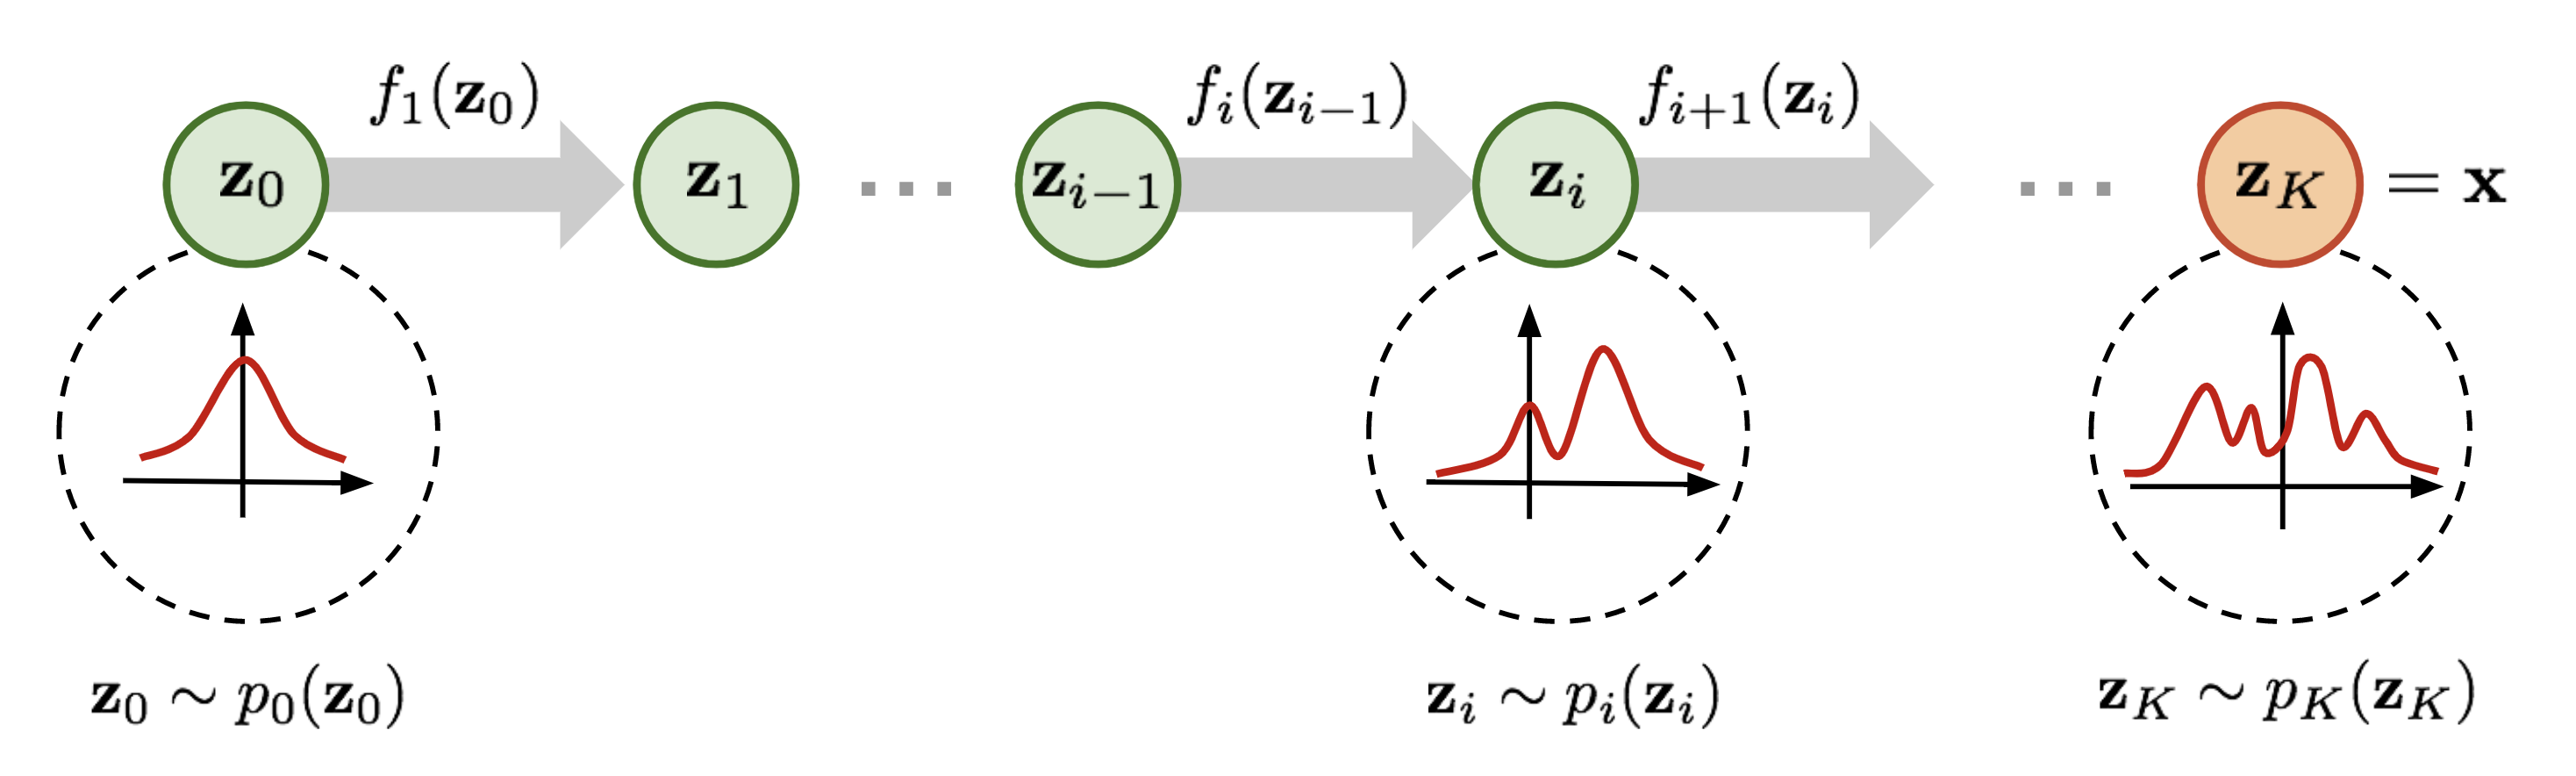
\includegraphics[width=0.85\textwidth]{img/normalizing-flow.png}
    \end{figure}}
    \only<4>{
    \textbf{Redes generativas antagónicas} (GAN)\\
    Las GANs son capaces de samplear nuevos puntos de datos al entrenar una red generadora que transforma ruido aleatorio en muestreos sintéticos, al mismo tiempo que ajusta una red discriminadora que distingue entre puntos reales y generados de manera sintética. Esto induce un bucle de retroalimentación (\textit{feedback loop}) que empuja el generador a crear puntos de datos cada vez más parecidos a los reales y más diversos. \footnote{Fuente de la imagen: \url{https://developers.google.com/machine-learning/gan/gan_structure}}
    \begin{figure}
        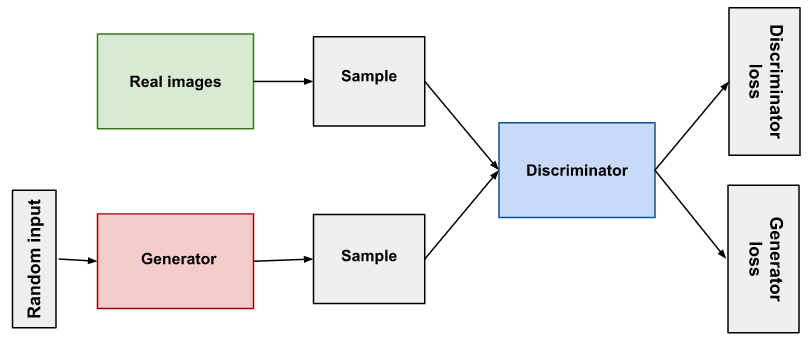
\includegraphics[width=0.8\textwidth]{img/gan.png}
    \end{figure}
    }
\end{frame}

\subsection{Taxonomía de Modelos Generativos}
\begin{frame}{La Taxonomía de Modelos Generativos}
    \centering
    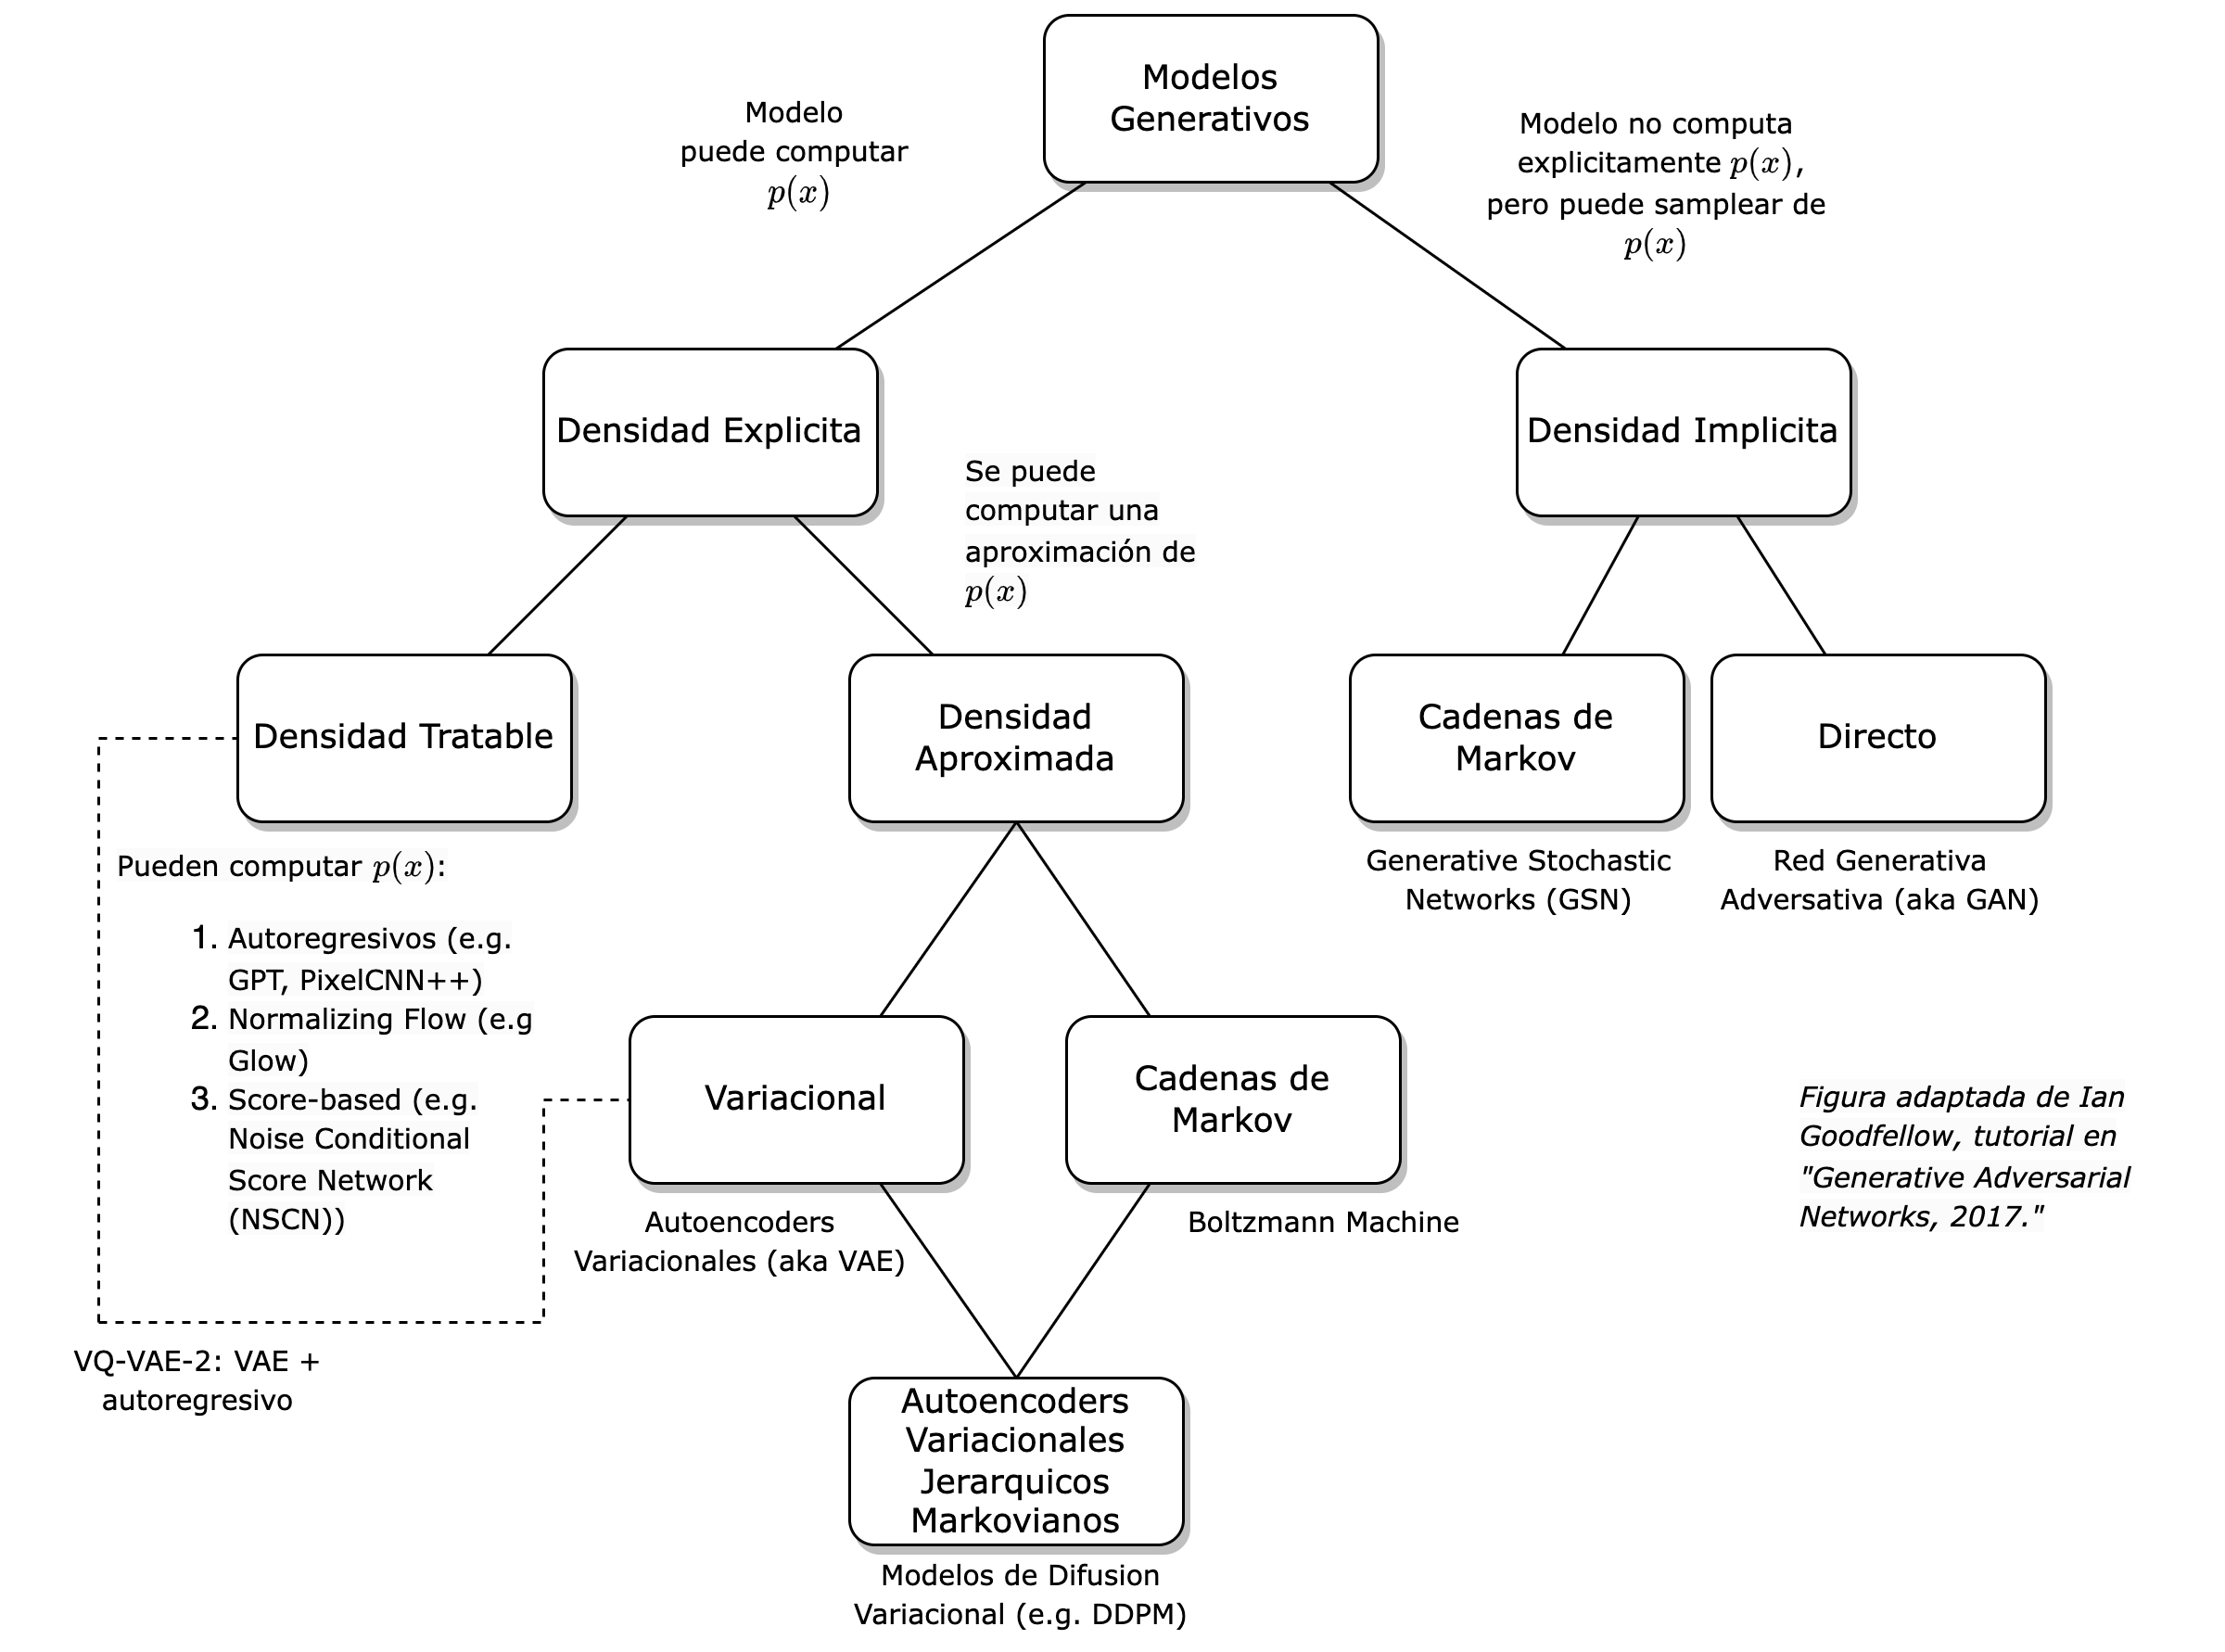
\includegraphics[width=0.9\textwidth]{diapositivas/img/taxonomy-generative-models.png}
\end{frame}


\section{Aplicaciones de Modelos Generativos}
\begin{frame}
    \frametitle{Tabla de contenidos}
    \tableofcontents[currentsection]
\end{frame}

\subsection{Modelos generativos y problemas inversos}
\begin{frame}{Modelos generativos y problemas inversos}
    \centering
    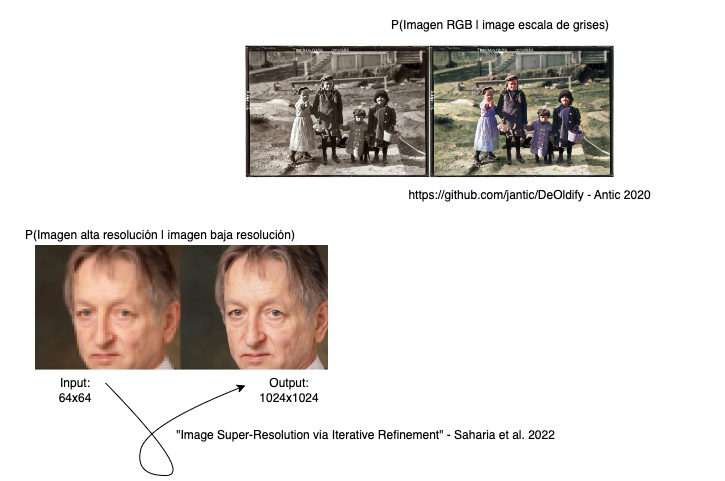
\includegraphics[width=0.9\textwidth]{diapositivas/img/inverse-problems.png}
\end{frame}


\subsection{Generación de imagen-a-imagen}
\begin{frame}{Generación de imagen-a-imagen}
    \centering
    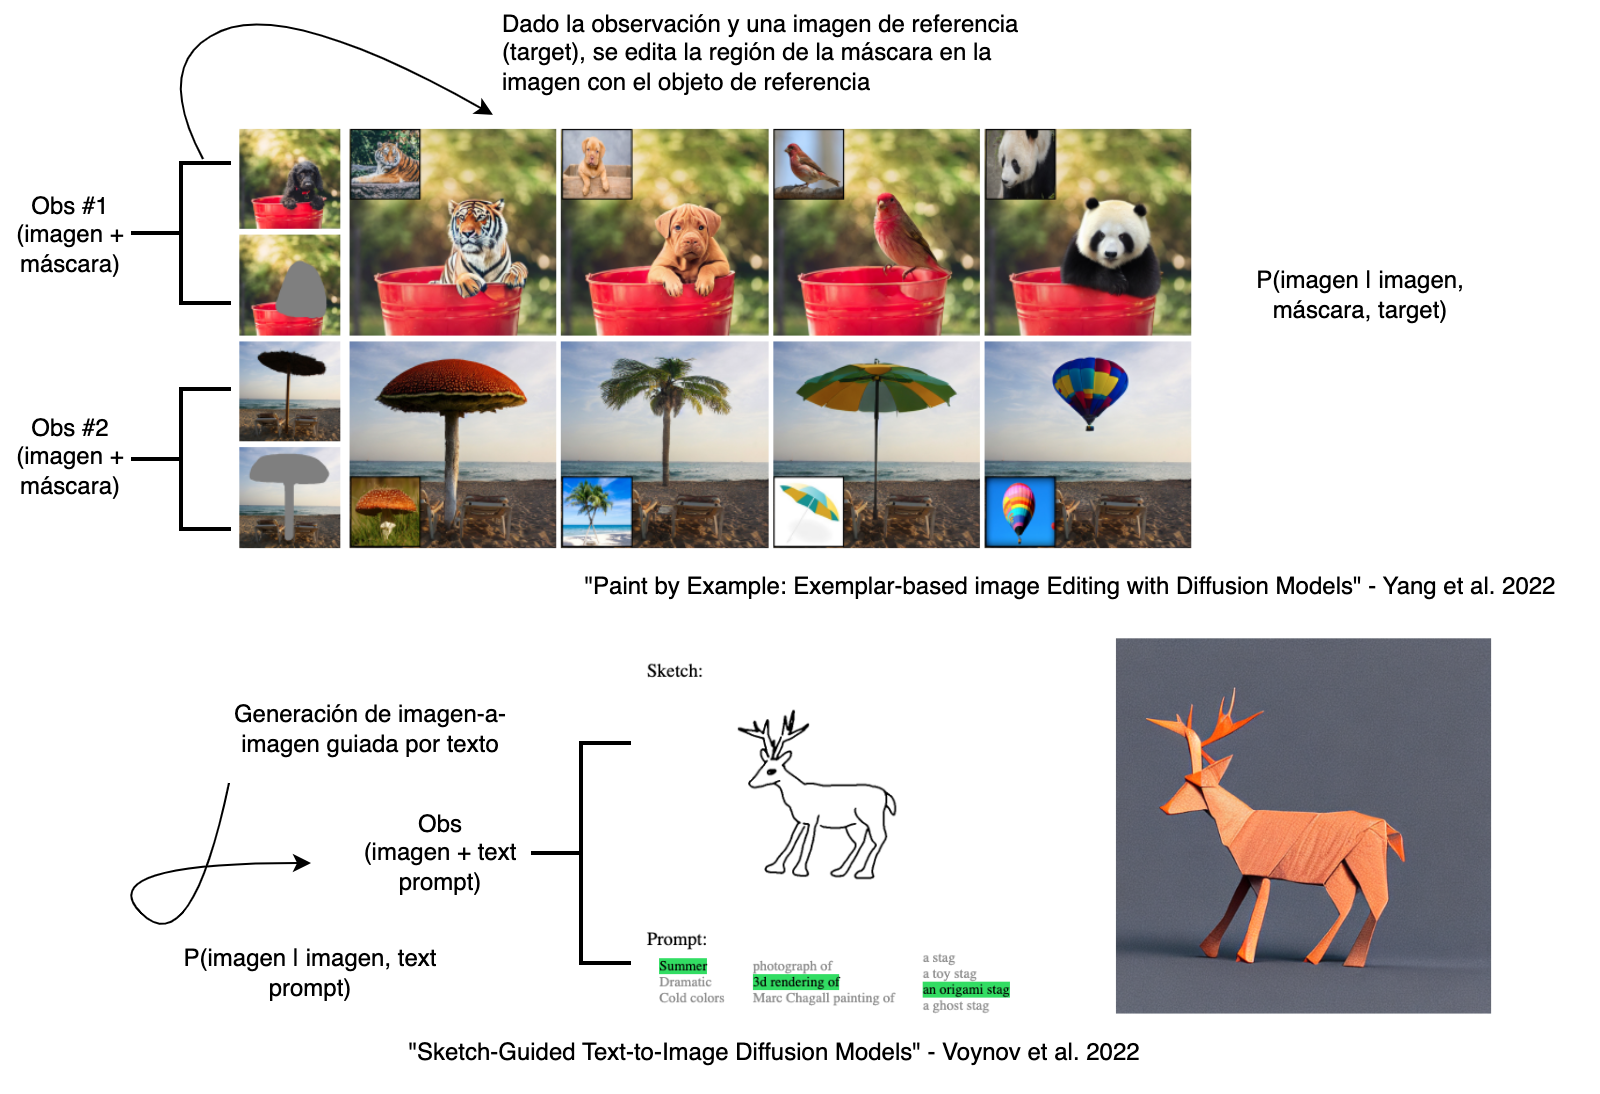
\includegraphics[width=0.9\textwidth]{diapositivas/img/img-to-img-dpi200.png}
\end{frame}

\subsection{Generación de imagen-a-imagen}
\begin{frame}{Generación de secuencias}
    \centering
    
\includegraphics[width=0.9\textwidth]{diapositivas/img/llm-task.png}
\end{frame}


\subsection{Aplicaciones en Industrias Creativas}
\begin{frame}
\frametitle{Aplicaciones de Modelos Generativos: Industrias Creativas}

\begin{columns}
\begin{column}{0.5\textwidth}
\textit{"No luz, no cámara, solo acción", \href{https://research.runwayml.com/gen2}{Runway, GEN-2}}
  \begin{itemize}
    \item \textit{Text-to-Video}
    \item \textit{Text + Image-to-Video}
    \item \textit{Image-to-Video}
    \item \textit{Stylization}
    \item \textit{Storyboard}
    \item \textit{Mask}
    \item \textit{Render}
  \end{itemize}
\end{column}
\begin{column}{0.5\textwidth}
  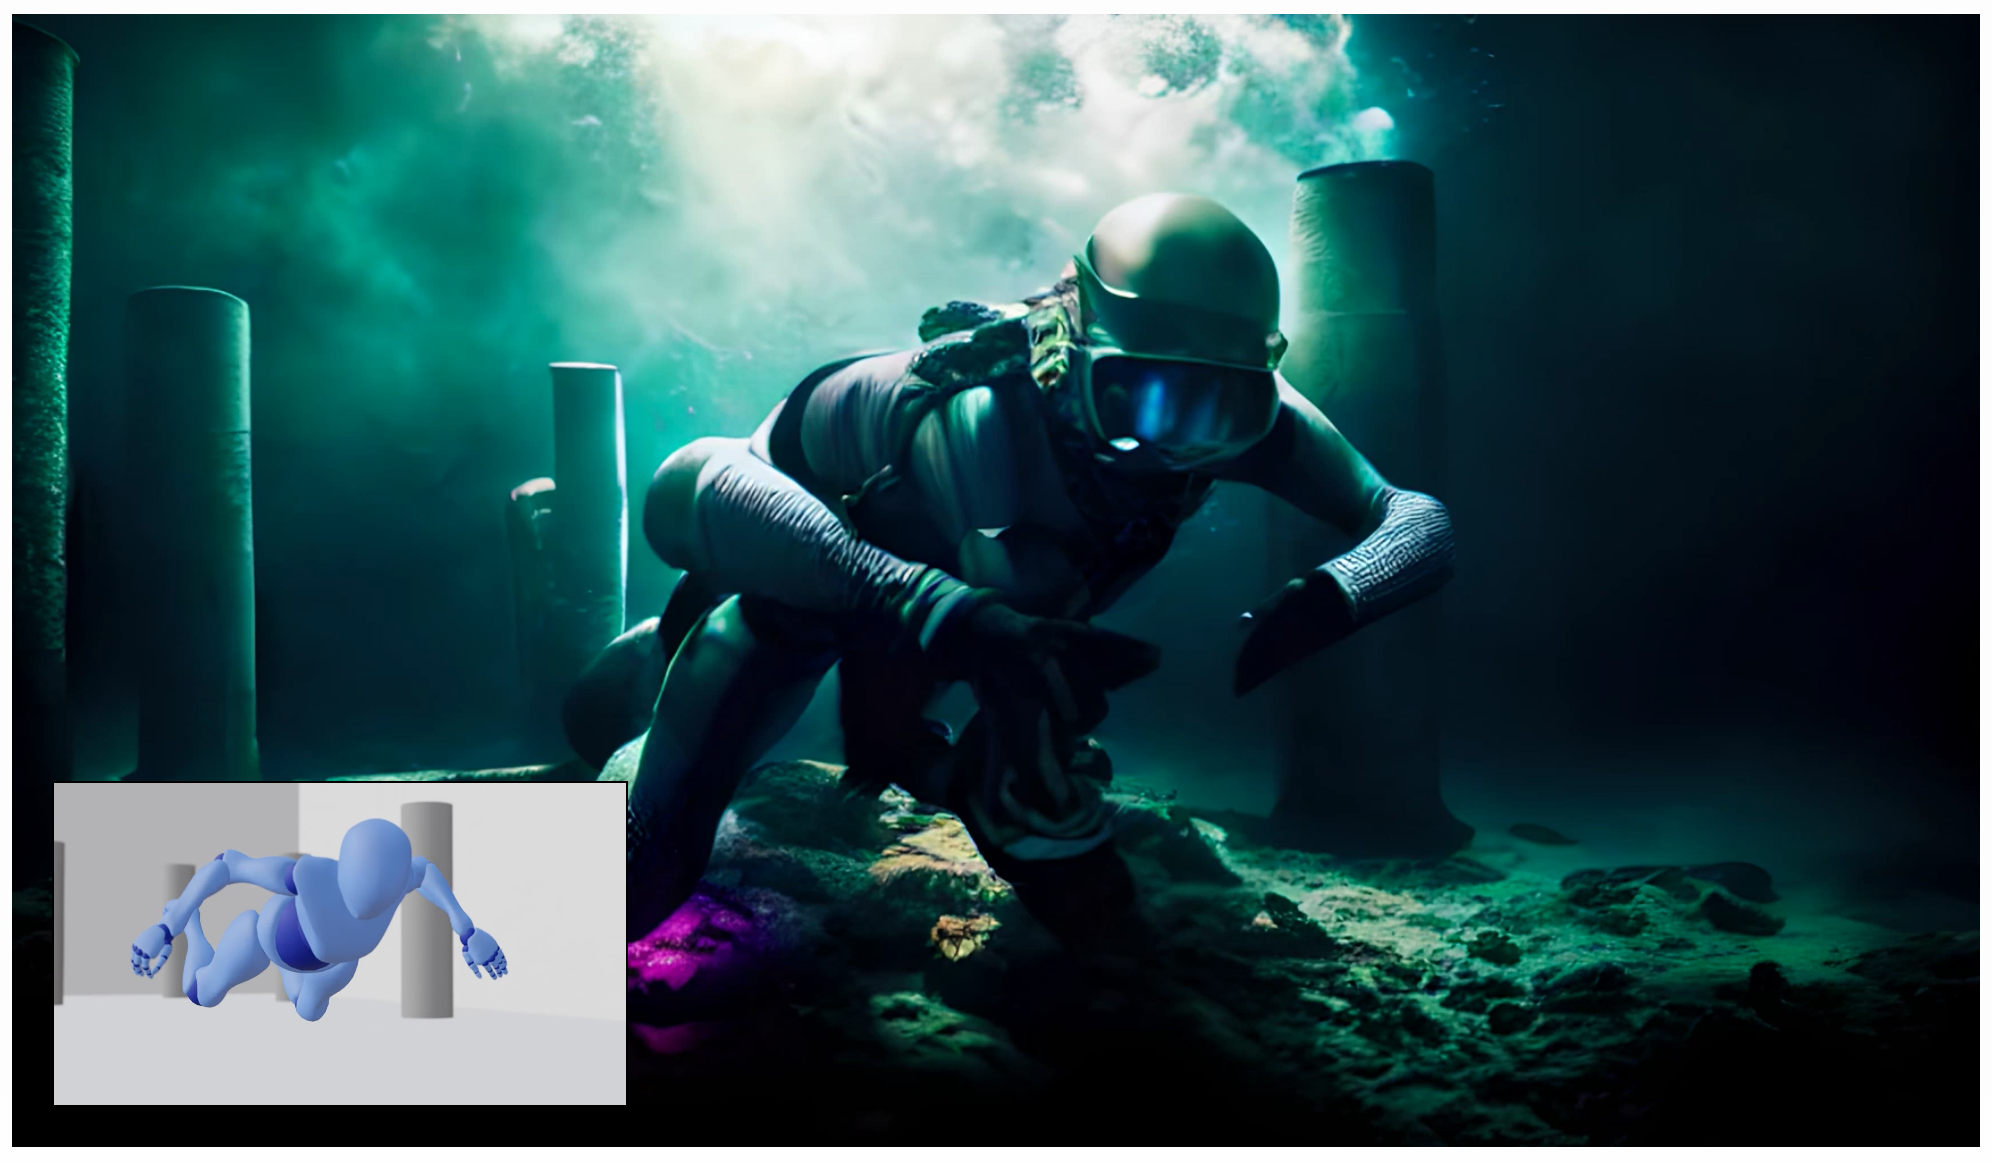
\includegraphics[width=\textwidth]{diapositivas/img/runaway-gen2-render.png}
\end{column}
\end{columns}
\end{frame}

\begin{frame}
  \titlepage
\end{frame}


%Quitar de comentarios apenas se agregue alguna referencia 
% \bibliography{../capitulos/referencias} %Bibliografía
% \bibliographystyle{apacite}

\end{document} 
